% ----------------------------------------------------
% Design
% ----------------------------------------------------
\documentclass[class=report,11pt,crop=false]{standalone}
% Page geometry
\usepackage[a4paper,margin=20mm,top=25mm,bottom=25mm]{geometry}
\usepackage{indentfirst}
% Font choice
\usepackage{lmodern}

% Use IEEE bibliography style
\bibliographystyle{IEEEtran}

% Line spacing
\usepackage{setspace}
\setstretch{1.20}

% Ensure UTF8 encoding
\usepackage[utf8]{inputenc}

% Language standard (not too important)
\usepackage[english]{babel}

% Skip a line in between paragraphs
\usepackage{parskip}

% For the creation of dummy text
\usepackage{blindtext}

% Math
\usepackage{amsmath}

\usepackage{enumitem}


% Header & Footer stuff
\usepackage{fancyhdr}
\pagestyle{fancy}
\fancyhead{}
\fancyhead[R]{\nouppercase{\rightmark}}
\fancyfoot{}
\fancyfoot[C]{\thepage}
\renewcommand{\headrulewidth}{0.0pt}
\renewcommand{\footrulewidth}{0.0pt}
\setlength{\headheight}{13.6pt}

% Epigraphs
\usepackage{epigraph}
\setlength\epigraphrule{0pt}
\setlength{\epigraphwidth}{0.65\textwidth}

% Colour
\usepackage{color}
\usepackage[usenames,dvipsnames]{xcolor}

% Hyperlinks & References
\usepackage{hyperref}
\definecolor{linkColour}{RGB}{77,71,200}%{0,144,208}%
\hypersetup{
    colorlinks=true,
    linkcolor=linkColour,
    filecolor=linkColour,
    urlcolor=linkColour,
    citecolor=linkColour,
}
\urlstyle{same}

% Automatically correct front-side quotes
\usepackage[autostyle=false, style=ukenglish]{csquotes}
\MakeOuterQuote{"}

% Graphics
\usepackage{graphicx}
\graphicspath{{Images/}{../Images/}}
\usepackage{makecell}
\usepackage{transparent}

% SI units
\usepackage{siunitx}

% Microtype goodness
\usepackage{microtype}

% Listings
\usepackage[T1]{fontenc}
\usepackage{listings}
\usepackage[scaled=0.8]{DejaVuSansMono}

% Custom colours for listings
\definecolor{backgroundColour}{RGB}{250,250,250}
\definecolor{commentColour}{RGB}{10, 204, 10}
\definecolor{identifierColour}{RGB}{0, 0, 255}%{196, 19, 66}
\definecolor{stringColour}{RGB}{255, 0, 255}
\definecolor{keywordColour}{RGB}{255,0,0}
\definecolor{lineNumbersColour}{RGB}{127,127,127}
\lstset{
  language=Python,
  captionpos=b,
  aboveskip=10pt,belowskip=10pt,
  backgroundcolor=\color{backgroundColour},
  basicstyle=\ttfamily,%\footnotesize,        % the size of the fonts that are used for the code
  breakatwhitespace=false,         % sets if automatic breaks should only happen at whitespace
  breaklines=true,                 % sets automatic line breaking
  postbreak=\mbox{\textcolor{red}{$\hookrightarrow$}\space},
  commentstyle=\color{commentColour},    % comment style
  identifierstyle=\color{identifierColour},
  stringstyle=\color{stringColour},
   keywordstyle=\color{keywordColour},       % keyword style
  %escapeinside={\%*}{*)},          % if you want to add LaTeX within your code
  extendedchars=true,              % lets you use non-ASCII characters; for 8-bits encodings only, does not work with UTF-8
  frame=single,	                   % adds a frame around the code
  keepspaces=true,                 % keeps spaces in text, useful for keeping indentation of code (possibly needs columns=flexible)
  morekeywords={*,...},            % if you want to add more keywords to the set
  numbers=left,                    % where to put the line-numbers; possible values are (none, left, right)
  numbersep=5pt,                   % how far the line-numbers are from the code
  numberstyle=\tiny\color{lineNumbersColour}, % the style that is used for the line-numbers
  rulecolor=\color{black},         % if not set, the frame-color may be changed on line-breaks within not-black text (e.g. comments (green here))
  showspaces=false,                % show spaces everywhere adding particular underscores; it overrides 'showstringspaces'
  showstringspaces=false,          % underline spaces within strings only
  showtabs=false,                  % show tabs within strings adding particular underscores
  stepnumber=1,                    % the step between two line-numbers. If it's 1, each line will be numbered
  tabsize=2,	                   % sets default tabsize to 2 spaces
  %title=\lstname                   % show the filename of files included with \lstinputlisting; also try caption instead of title
}

% Caption stuff
\usepackage[hypcap=true, justification=centering]{caption}
\usepackage{subcaption}

% Glossary package
% \usepackage[acronym]{glossaries}
\usepackage{glossaries-extra}
\setabbreviationstyle[acronym]{long-short}

% For Proofs & Theorems
\usepackage{amsthm}

% Maths symbols
\usepackage{amssymb}
\usepackage{mathrsfs}
\usepackage{mathtools}

% For algorithms
\usepackage[]{algorithm2e}

% Spacing stuff
\setlength{\abovecaptionskip}{5pt plus 3pt minus 2pt}
\setlength{\belowcaptionskip}{5pt plus 3pt minus 2pt}
\setlength{\textfloatsep}{10pt plus 3pt minus 2pt}
\setlength{\intextsep}{15pt plus 3pt minus 2pt}

% For aligning footnotes at bottom of page, instead of hugging text
\usepackage[bottom]{footmisc}

% Add LoF, Bib, etc. to ToC
\usepackage[nottoc]{tocbibind}

% SI
\usepackage{siunitx}

% For removing some whitespace in Chapter headings etc
\usepackage{etoolbox}
\makeatletter
\patchcmd{\@makechapterhead}{\vspace*{50\p@}}{\vspace*{-10pt}}{}{}%
\patchcmd{\@makeschapterhead}{\vspace*{50\p@}}{\vspace*{-10pt}}{}{}%
\makeatother
\makenoidxglossaries


\newacronym{fm}{FM}{Frequency Modulation}
\newacronym{am}{AM}{Amplitude Modulation}
\newacronym{em}{EM}{electromagnetic}
\newacronym{iq}{IQ}{In-phase and Quadrature}


\newacronym{dft}{DFT}{Discrete Fourier Transform}
\newacronym{idft}{IDFT}{Inverse Discrete Fourier Transform}
\newacronym{fft}{FFT}{Fast Fourier Transform}
\newacronym{ifft}{IFFT}{Inverse Fast Fourier Transform}

\newacronym{df}{DF}{Direction Finding}
\newacronym{rdf}{RDF}{Radio Direction Finding}
\newacronym{AoA}{AoA}{Angle of Arrival}
\newacronym{rf}{RF}{Radio Frequency}
\newacronym{sdr}{SDR}{Software-Defined Radio}
\newacronym{pd}{PD}{Phase-Difference}
\newacronym{vhf}{VHF}{Very High Frequency}
\newacronym{MHz}{MHz}{Megahertz}
\newacronym{db}{dB}{decibel}
\newacronym{dbm}{dBm}{Decibel-milliwatts}
\newacronym{rx}{Rx}{Receiver}
\newacronym{tx}{Tx}{Transmitter}
\newacronym{dsp}{DSP}{Digital Signal Processing}
\newacronym{vor}{VOR}{Very High Frequency Omnidirection Range}
\newacronym{gps}{GPS}{Global Position System}
\newacronym{adf}{ADF}{Automatic Direction Finders}
\newacronym{ndb}{NDB}{Non-Directional Beacon}
\newacronym{sm}{S meter}{Signal Strength Meter}
\newacronym{tdoa}{TDOA}{Time Difference of Arrival}
\newacronym{ham}{HAM}{an informal name for an amateur radio operator}
\newacronym{wbfm}{WBFM}{Wideband Frequency Modulation}
\newacronym{if}{IF}{Intermediate Frequency}
\newacronym{lp}{LP}{Low Pass}
\newacronym{API}{API}{Application Programming Interface}
\newacronym{fpga}{FPGA}{Field-Programmable Gate Array}
\newacronym{bw}{BW}{Bandwidth}
\newacronym{adc}{ADC}{Analog-to-digital converter}
\newacronym{tv}{Tv}{Television}
\newacronym{ai}{AI}{Artificial Intelligence}
\newacronym{lo}{LO}{Local Oscillator}
\newacronym{icasa}{ICASA}{Independent Communications Authority of South Africa}
\newacronym{usb}{USB}{Universal-serial Buss}
\newacronym{os}{OS}{Operating System}
\newacronym{mimo}{MIMO}{Mutliple input, Multiple output}
\newacronym{vna}{VNA}{Vector Network Analyser}
\newacronym{mse}{MSE}{Mean Squared Error}
\newacronym{SNR}{SNR}{Signal-to-Noise Ratio}

\begin{document}
\ifstandalone
\tableofcontents
\fi
% ----------------------------------------------------

\chapter{Implementation of Direction Finding\label{ch:design}}
\epigraph{``Between stimulus and response there is a space. In that space is our power to choose our response. In our response lies our growth and our freedom.''}
    {\emph{---Viktor E. Frankl}}
\vspace{0.5cm}
% ----------------------------------------------------

%---------------------------------
% Intro
%---------------------------------
The following chapter builds on the Design Methodology and details the core components of the project, both Hardware and Software. The fundamental aim is to prototype and validate a \gls{rdf} system, with proof that through \gls{pd} calculations, an \gls{AoA} can be estimated. Fortunately, the previous Chapters have outlined the implementation, as well as the theoretical understanding for the project, including what falls outside of the scope and thus not implemented or tested. 

This chapter begins with the first stage of implementation: to use non-noisy, simulated reference data to achieve the working algorithms of the project. This allowed for the algorithms to subsequently be implemented into the prototype with the LimeSDR, \gls{rx} antennas and tested on real-world data. 

Following this, a high-level overview of the systems and the contained components are selected and connected as per the Methodology of the project. Each subsequent section dives deeper into the individual blocks of the project, giving the necessary code snippets and diagrams. All variable names match directly to the variables used in the \textsc{Python} code from this project. 

The final section of this chapter deals with the validation of working hardware and portions of the software. 
%---------------------------------
% Sim
%---------------------------------
\section{Simulation Design}\label{sec:Design/SimulationDesign}
In order to test the theoretical working of a \gls{pd} calculation, before development in hardware, the following simulation was conducted as validation.

\subsection{Language and Environment}
In the context of this project, \textsc{Julia} was chosen as the programming language for the simulation. Not only did this allow for the development of a new skill, but the \textsc{Julia} language is highly suited to applications of this nature. \textsc{Julia} was specifically designed for high-speed calculations, \gls{dsp} and machine learning. Based on \textsc{Python}, \textsc{Julia} is a \emph{typeless} \footnote{This is not strictly true. Every object most certainly has a type, however, due to the lack of type declarations, there is no instruction to the compiler about types and therefore deemed typeless.} language. However differing from \textsc{Python}, \textsc{Julia} features an 'on the fly' compiler, making the performance comparable to C++. Additionally, \textsc{Juilia} features a highly sophisticated back-end for plotting, while still maintaining a lightweight codebase

For ease of development and testing, this simulation was designed in a Jupyter Notebook, using a \textsc{Julia} kernel. Jupyter Notebooks are incredibly powerful, allowing sections of code to be run individually and allow for professional, interactive and clean projects. The Notebook is run off a local \textsc{Python} server in the web browser. 

\subsection{Overview}
Figure \ref{fig:phase-change} shows the simulated environment for the antenna array and transmission source using euclidean coordinates. The first step of the simulation is to produce a pure $sin$ wave of 150MHz as the transmission source. For the purposes of validation, this simulation was kept noise-free.

\begin{figure}[h]\centering
    \subfloat[\emph{Julia} code]{\label{a}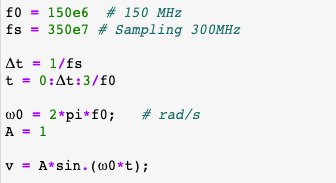
\includegraphics[width=.4\linewidth]{Images/plots/sim-tranmission-code.png}}
    \subfloat[Signal Produced]{\label{a}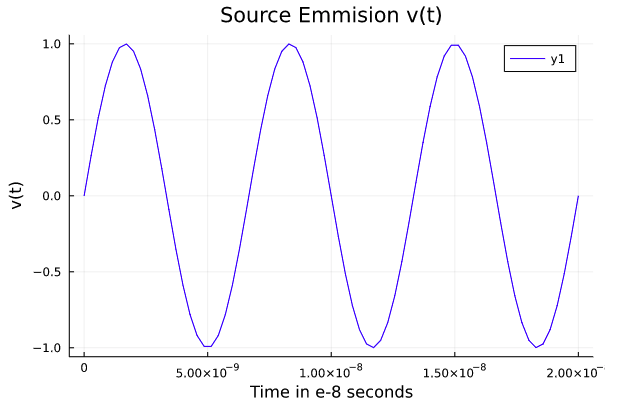
\includegraphics[width=.4\linewidth]{Images/plots/sim-tranmission.png}}\hfill
     \caption{Simulation transmission source \emph{Julia} code and produced signal}
    \label{fig:sim-transmission}
\end{figure}

\subsection{Simulated Phase Delay}
In order to simulate a change in phase, due to relative positions of the transmission source to the \gls{rx} antenna, the distance was calculated between the emitted signal and the \gls{rx} antenna, depending on the euclidean coordinates of the elements. With the distance known, and recalling \gls{em} propagate at the speed of light, a phase delay is added to signal $v1$ in listings \ref{ls-41} and \ref{ls-Phase-delay}.

\noindent\hspace{0.03\linewidth}\begin{minipage}[t]{.48\linewidth}\centering
\begin{lstlisting}[caption={Distance between emitted signal and antenna element}, label={ls-41}]
# Antenna
ax = [-0.5,0.5], ay = [0,0]
# Source
sx = [1000], sy = [1000]
# Antenna 1
d1 = sqrt.((sx[1]-ax[1])^2+(sy[1]-ay[1])^2)
\end{lstlisting}
\end{minipage}%
\hspace{0.5cm}
\begin{minipage}[t]{.4\linewidth}\centering
\begin{lstlisting}[language=Python, caption=Adding of a phase delay based off distance between source and \gls{rx} antenna, label=ls-Phase-delay]
# Calculating time delay
c = 3e8
t1 = d1/c
# Adding phase delay and FFT
v1 = A*sin.(w0*t.-t1);
V1 = fft(v1)
\end{lstlisting}
\end{minipage}

With complex arrays $V1$ and $V2$, now in the frequency domain representing the phase delayed, \gls{rx} signal, the phase of each signal can be extracted by first finding the index of the magnitude of the signal. 
In \textsc{Julia}, listing \ref{ls-julia-max} extracts both the index and maximum value from an array. 

\begin{lstlisting}[language=Python, caption=Extracting Index of Maxiumum magnitude value from FFT of \gls{rx} signal, label=ls-julia-max]
maxsignal_1 = findmax(abs.(V1)) #Returns [maximum value of magnitude, index which it occurs]
maxsignal_2 = findmax(abs.(V2)) #Returns [maximum value of magnitude, index which it occurs]
\end{lstlisting}

The complex numbers $p1$ and $p2$ represent the value of the phasor that represents the signal of interest

\begin{lstlisting}[language=Python, caption=Phasor extraction of signal of interest]
p1 = V1[maxsignal_1]
p2 = V2[maxsignal_2]
\end{lstlisting}
From which the phase of the signal can be extracted in two different ways:

\noindent\hspace{0.03\linewidth}\begin{minipage}[t]{.48\linewidth}\centering
\begin{lstlisting}[language={Python}, caption={Phase extraction using angle() and \gls{pd}}, label={ls-distance}]
phase1 = angle(p1)
phase2 = angle(p2)
phase_diff = phase2 - phase1
\end{lstlisting}
\end{minipage}%
\hspace{0.5cm}
\begin{minipage}[t]{.4\linewidth}\centering
\begin{lstlisting}[language=Python, caption=\gls{pd} calculation using using conjugate symmetry]
Z = p1 * conj(p2)
# in rads
phase_diff = angle(Z) 
\end{lstlisting}
\end{minipage}

This basic simulation proved that extraction of the \gls{pd} was possible, and thus the simulation was looped for testing purposes to produce calculated \gls{AoA}, reported on in Chapter \ref{ch:results}.


%---------------------------------
% System Design   
%---------------------------------
\section{System-Level Design}\label{sec:Design/SystemDesign}
The prototype system built for this project is based on Chapter \ref{ch:meth}, and adheres to the device requirements. This section details the hardware components used and an overview of the system is shown in Figure \ref{fig:system}

\begin{figure}[h]
    \centering
    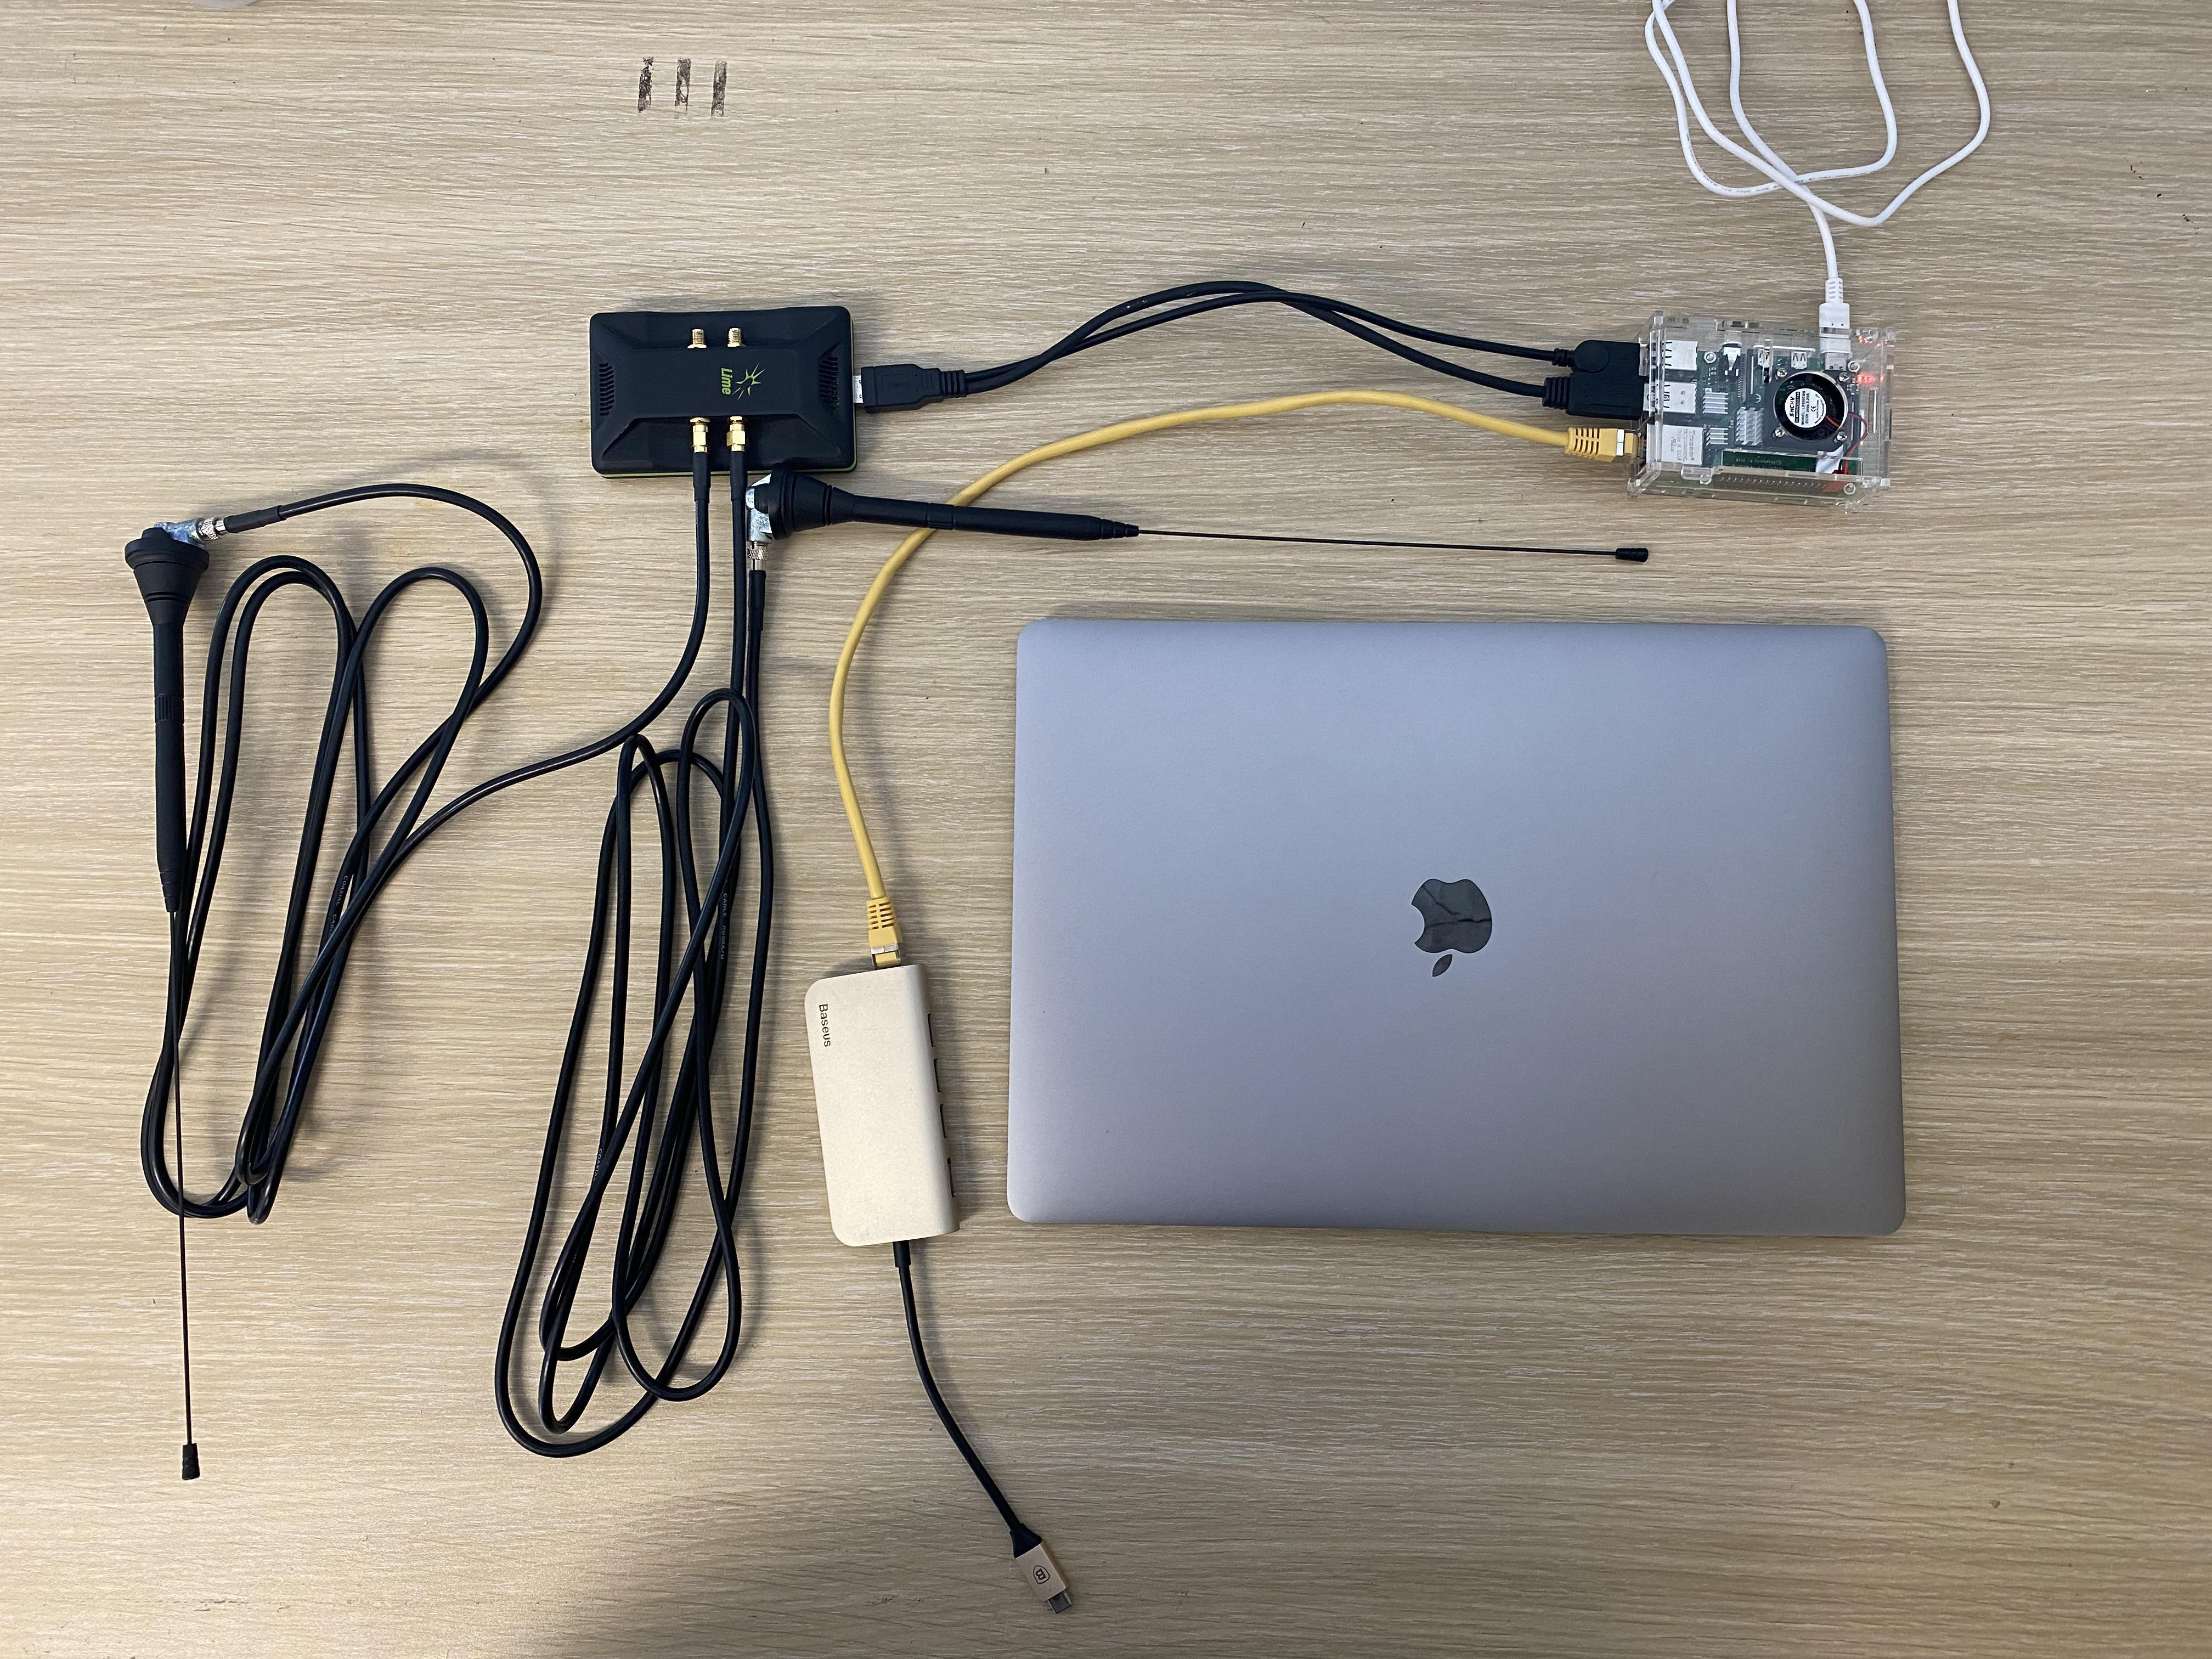
\includegraphics[width=0.6\linewidth, height=6cm]{Images/diagrams/system.jpg}
    \caption{Overview of system hardware used for this project}
    \label{fig:system}
\end{figure}

\subsection{Raspberry Pi}
The Raspberry Pi Model 4 B was used for this project due to its low cost, portability and frankly well-suited hardware specifications. The Host computer needed to control the \gls{sdr} had to be based of a Linux \gls{os}, and the PiSDR \footnote{PiSDR is a modified version of the default Raspbian image with the latest SDR software and drivers for multiple devices pre-installed.} image available for this device was a benefit. The MacBook computer was merely a screen for the Pi during testing.  The Raspberry Pi can be summarised in table \ref{tab:pi}.

\vspace{0.5cm}
\begin{center}
    \begin{tabular}{c|c}
        Device Requirement & Raspberry Pi 4 specifications  \\
        \hline
        \gls{os} & PiSDR, Linux \\
        CPU & 64-bit Quad core Cortex-A72 \@ 1.5GHz \\
        Memory & 4GB LPDDR4-3200 SDRAM\\
        \gls{usb} & 2 USB 3.0 ports; 2 USB 2.0 ports\\ 
        Output Power & 1.2A \gls{usb} output\\
    \end{tabular}
    \captionof{table}{Device summary of the Pi4, with consideration of the hardware requirements for the project \label{tab:pi}}
\end{center}

\subsubsection{Raspberry PiSDR image}
The \gls{os} used for this project is PiSDR. PiSDR is a modified version of the default Raspbian image with the latest SDR software and drivers for multiple devices already pre-installed. PiSDR is provided open-source by Luigi Cruz on his \href{https://github.com/luigifcruz}{GitHub Page}.

Notably, this image comes with support for both the LimeSDR device and LimeSuite itself. 

\subsubsection{VNC Viewer}
During testing, VNC Viewer was used for connecting to the Raspberry Pi device. The connection was made using Gigabit Ethernet cable directly to the port on the Raspberry Pi. This was sufficient for the prototype, however a LED touchscreen for the Pi would be beneficial in future use. 

\subsection{LimeSDR}
The \gls{sdr} device used in this project is the LimeSDR-USB, as depicted in Figure \ref{fig:lime-board}. A complete feature list of the board can be found in Appendix \ref{Appendix-B}, however, noting here how this \gls{sdr} is well suited to the device requirements of this project as listed in table \ref{tab:limesdr} \cite{myriad}.

\begin{figure}[h]
    \centering
    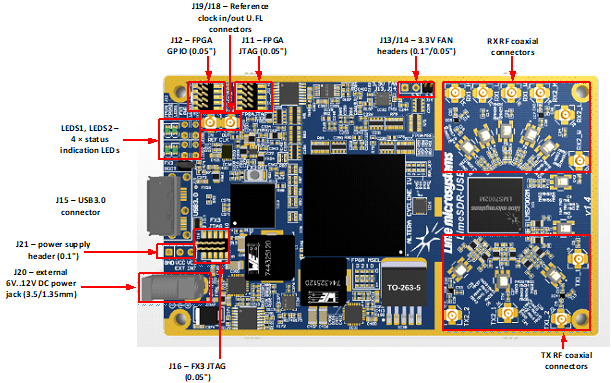
\includegraphics[width=0.8\textwidth]{Images/diagrams/LimeSDR-USB.png}
    \caption{An overview of the LimeSDR board}
    \label{fig:lime-board}
\end{figure}

\begin{center}
    \begin{tabular}{|p{0.45\textwidth} | p{0.55\textwidth}|}
        \hline
        \textbf{Hardware Feature} & \textbf{LimeSDR} \\
        \hline
        \hline
        \gls{rf} Transceiver & LMS7002M MIMO FPRF \\
        \hline
        Available Channels & 2×2 MIMO, (6 RX, 4 TX) \\
        \hline
        Clock System & 30.72MHz VCTCXO (precision: ±1 ppm initial, ±4 ppm stable) \\
        \hline
        Frequency Range & 100 kHz – 3.8 GHz\\
        \hline
        Bandwidth & 61.44 MHz \\
        \hline
        \gls{usb} Interface & 2X Cypress USB 3.0, \gls{usb}3.0 data transfer, 2.0 power \\
        \hline
        \gls{adc} & 4X integrate 12-bit \gls{adc}\\
        \hline
        \gls{fpga} & Cyclone IV EP4CE40F23\\
        \hline
    \end{tabular}
    \captionof{table}{Key hardware specifications of the LimeSDR device for the project   \label{tab:limesdr}}
\end{center}

\subsection{LimeSDR Interfacing}
Both the SoapySDR \gls{API} as well as the LimeSuite Driver came pre-installed on the PiSDR \gls{os}. Both interfacing options were utilised: the LimeSuite driver for generating the \emph{register configuration (init) file} and the SoapySDR \gls{API} wrapper to interface with GNU Radio. 

A full guide for installation is found at MyRiadRF \cite{myriad}, however noting here how the interfacing options utilised are implemented in Figure \ref{fig:limeSDR-interfacing-soapy}.  

Thus, connections, as seen in  Listing \ref{lst-gnu-init}, are now possible and implemented for the project.

\subsection{Antenna}
For this project, two 32.5cm monopole antennas were used due to the availability within the University. The development of a correctly matched antenna was out of scope for this project, and while not ideally suited the antenna were still capable for the prototype systems validation.

\begin{equation*}
\begin{split}
    \lambda & = \frac{c}{frequency} \\
    & = \frac{3 \times 10^8}{150 \times 10^6} \\
    & = 2 m 
\end{split}
\end{equation*}

\textbf{$\therefore \frac{1}{4} \times \lambda$ = 50cm  would have been the ideal antenna length.}


The spacing of antenna was adjusted when validating of \gls{fm} Radio stations, however, Figure \ref{array} shows the orientation of the array used for testing at 150MHz. 
\begin{figure}[h]\centering
    \subfloat[Physical geometry of the antenna array used for this project.]{\label{array}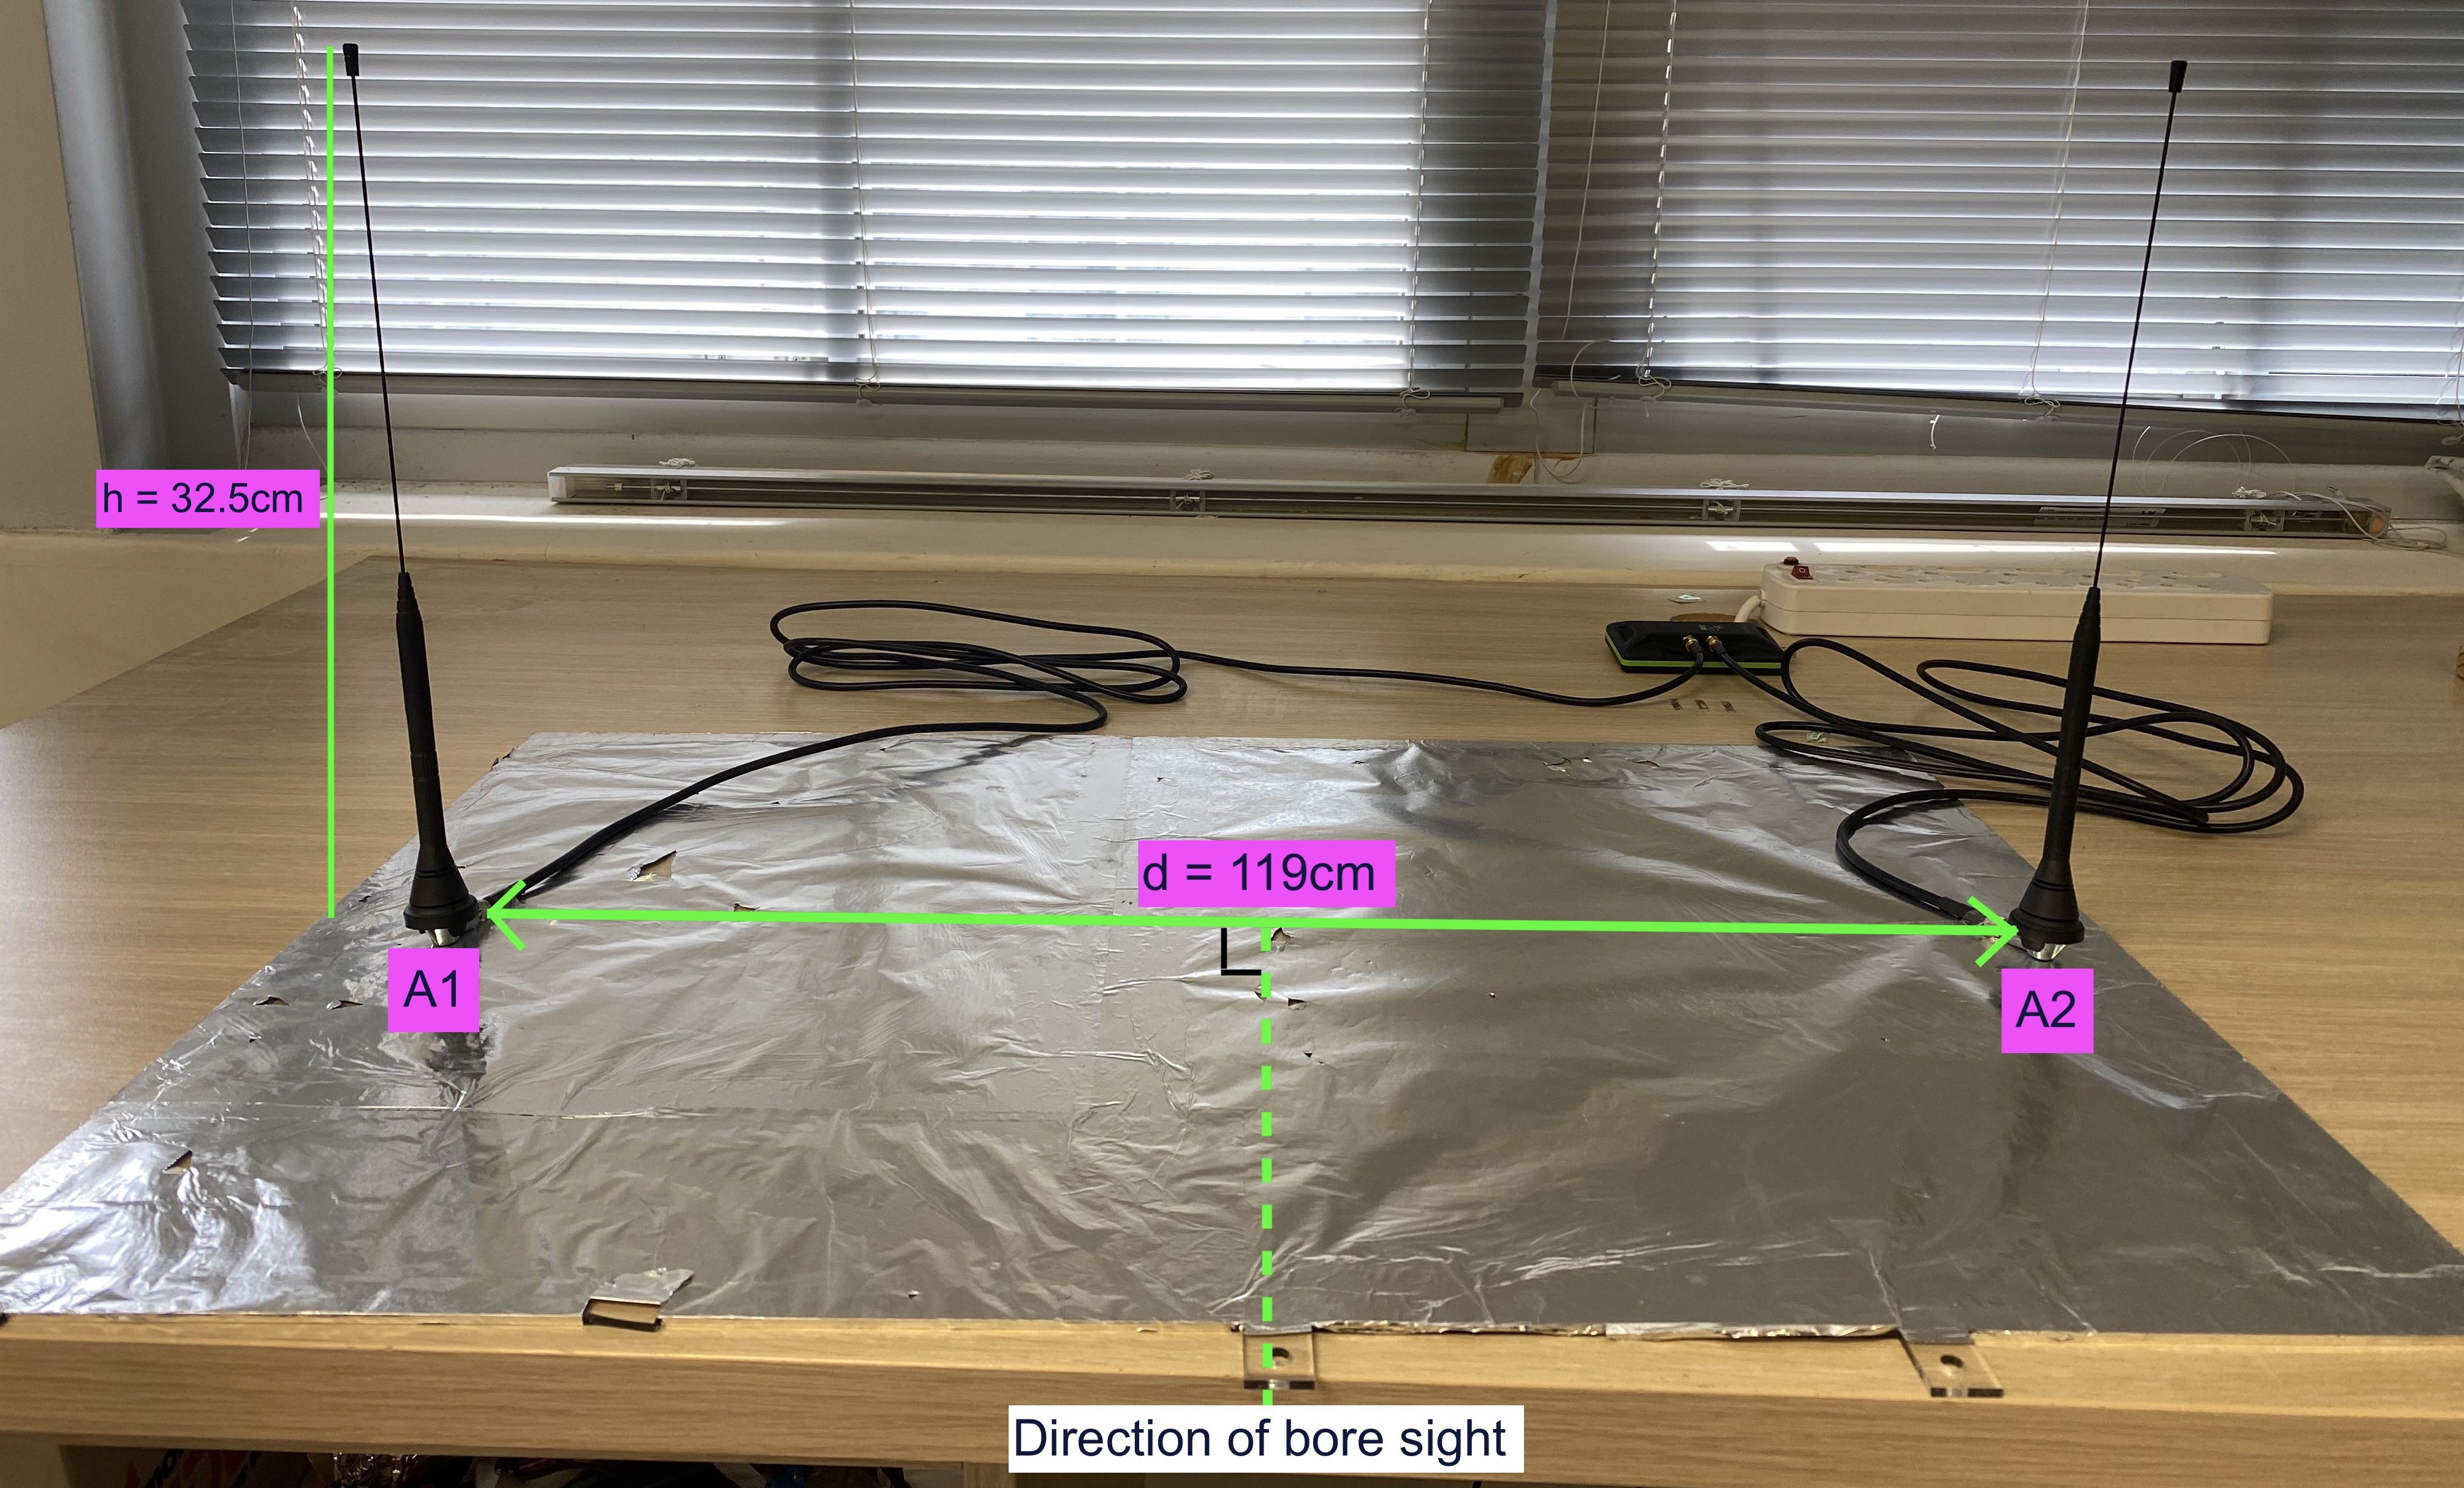
\includegraphics[width=.53\linewidth]{Images/diagrams/antenna-array.jpg}}\hspace{.5cm}
    \subfloat[S11 Parameter analysed from \gls{vna} of the antenna used in this project]{\label{a}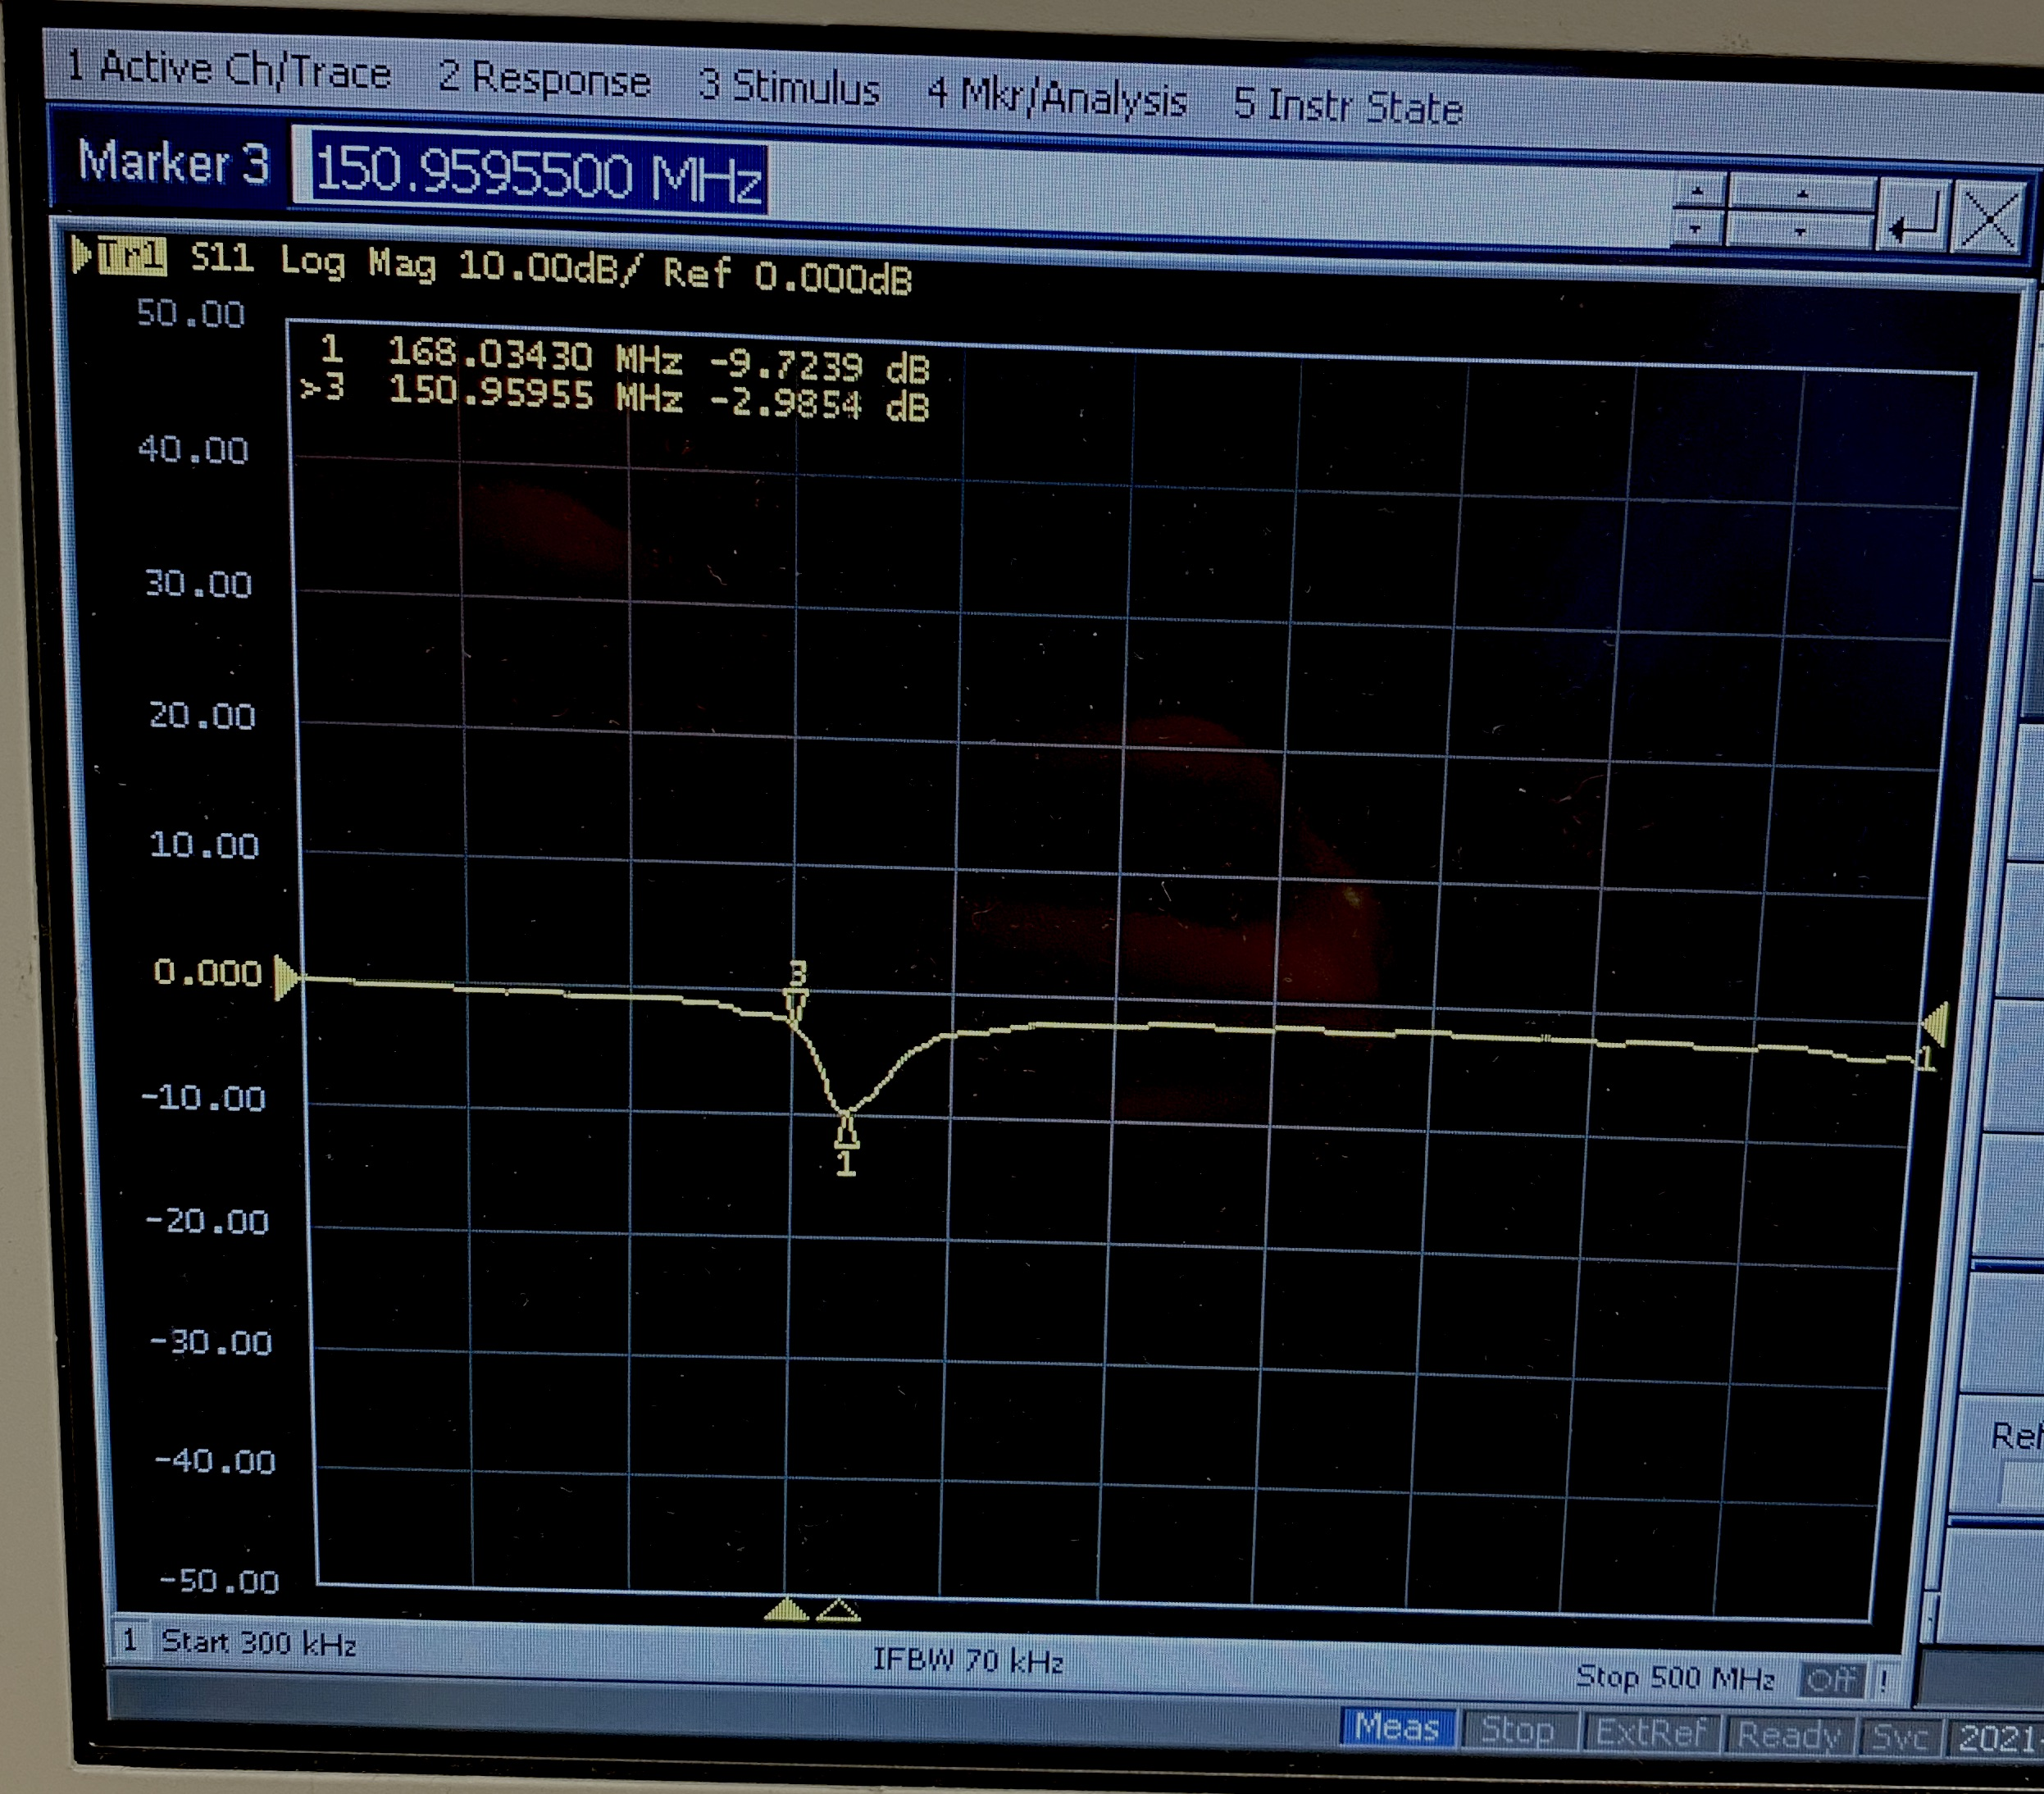
\includegraphics[width=.38\linewidth]{Images/diagrams/s-params.jpg}}\hfill 
    \caption{Further details into the parameters and dimensions for the antenna of this project}
    \label{fig:antenna}
\end{figure}

%---------------------------------
% Hardware design 
%---------------------------------
\section{Hardware Design}\label{sec:Design/HardwareDesign}
The following section of this report deals with the configuration of the hardware components used for the project. Where changes to the default behaviour of a device are made, it is documented below. 

\subsection{LimeSDR Initialisation}
It is important to note that the internal hardware configurations within the LimeSDR are volatile. This means that when the power is cycled to the \gls{sdr}, the internal configurations are reset. As a result, each time the board is powered on, either the LimeSuiteGUI is needed to configure the registers and settings, or an initialisation bit file can be flashed. 

The LimeSuiteGUI provides default \gls{API} functions that enable fine control of the board internal hardware configuration. 

Environments like GNU Radio do not allow for control on this level of the \gls{sdr} board, but instead, run the initialisation file after connecting to the board. 

Table \ref{tab:lime-api} contains the \gls{API} functions used to generate the limesdr\_init.ini bit file. 

\begin{table}[]
    \centering
    \begin{tabular}{|m{4.1cm} | m{7cm}| m{5cm} | }
        \hline
        \multicolumn{1}{|c}{\textbf{\gls{API} Function}} & \multicolumn{1}{|c|}{\textbf{Description}} & \multicolumn{1}{c|}{\textbf{Paramters}} \\
        \hline
        \hline
        LMS\_EnableChannel & Set \gls{rx}/ \gls{tx} for channel port & RX/TX | Chanel No | Enabled/Disabled \\
        \hline
        LMS\_SetSampleRate & Set sampling rate for all channels. Max DAC sampling rate of the RF chip is 640MHz. & MHz \\
        \hline
        LMS\_SetLOFrequency & Set the frequency of \gls{lo} for give channel index and type & RX/TX | Chanel No | MHz \\
        \hline
        LMS\_SetAntenna  & Select gain mode for specific channel & RX/TX | Chanel No | Gain Mode \\
        \hline
        LMS\_SetGaindB & Set the system gain, modified by NormazlizedGain & RX/TX | Chanel No | dB value \\
        \hline 
        LMS\_SetNormalizedGain & Set the gain of the channel index,  \emph{pGain} parameter  &  RX/TX | Chanel No | value between 0 and 1\\ 
        \hline
        
    \end{tabular}
    \caption{A table of the LimeSuiteGUI \gls{API} used to create the bit file for this project}
    \label{tab:lime-api}
\end{table}

Additional information about all available \gls{API} functions courtesy of MyRiadRF can be found at the official \href{https://github.com/myriadrf/LimeSuite/tree/master/src/examples}{GitHub Page} 

\subsection{SDR settings}
The result of running the above mentioned \gls{API} is the settings of the LimeSDR board for validation shown in \ref{tab:sdrsetting}. These settings while functionally, are not optimised as stated in Chapter \ref{ch:intro}, and finer tuning of the parameters may have resulted in better phase results. However, time and scope constraints for the project prevented this. 

\begin{table}[h]
    \centering
    \begin{tabular}{c|c}
        \textbf{Hardware Parameter} & \textbf{Value used}  \\
        \hline
        \gls{rx} channel 0  &  Enabled, LNAL\\
        \gls{rx} channel 1  & Enabled, LNAL\\
        Sample Rate & 10MSps\\
        \gls{lo} Frequency & 148MHz \\
        Channel gain & 35dB both channels\\
    \end{tabular}
    \caption{LimeSDR internal hardware parameter settings used for the project}
    \label{tab:sdrsetting}
\end{table}
With the \gls{lo} set at 148MHz, and the project centred around the 150MHz band, the difference frequency used for sampling is 2MHz, and with a sample rate of 10MSps, the Nyquist sampling theorem is more than satisfied. 

Note, however, that the sample rate was adjusted for when testing on 89MHz vs 150MHz bands.

\subsection{Synchronisation}
As discussed in section \ref{sec:Software-Meth}, the GNU Radio scheduler and \emph{work} functions are responsible for the synchronisation of the two \gls{rf}. 

The internal hardware of the LMS7002M \gls{fpga} is shown in Figure \ref{fig:lms7002}, and the scheduler has been shown in Figure \ref{fig:gnu-scheduler} previously. Listing \ref{lst-work} shows the function calls from the \emph{main()} \textsc{Python} function which is handled by the GNU Radio scheduler. \emph{tb = top\_block\_cls()} is the \emph{work()} function in this application.

\begin{figure}[h]
    \centering
    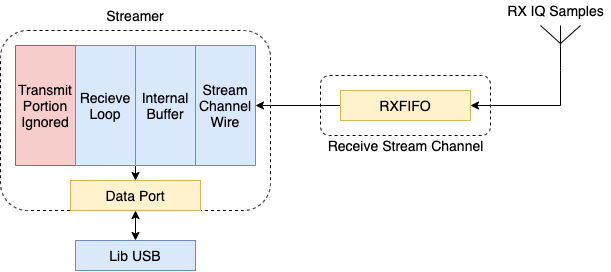
\includegraphics[width=0.8\textwidth]{Images/diagrams/limesdr-mem.png}
    \caption{Memory transfer via USB Port from LimeSDR, adapted from \cite{gnu-delays}}
    \label{fig:lime-mem}
\end{figure}

\begin{figure}[h]
    \centering
    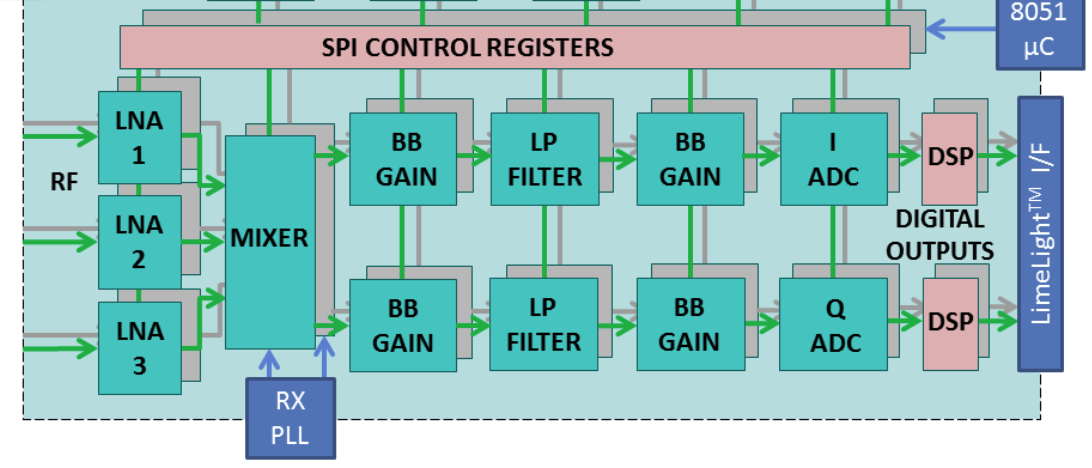
\includegraphics[width=0.8\textwidth]{Images/diagrams/lms7002.png}
    \caption{LMS7002M FPGA, with separate RF channels for built-in synchronisation \cite{myriad}}
    \label{fig:lms7002}
\end{figure}

\begin{lstlisting}[language={Python}, caption={Function calls made from \emph{main()} function to the \emph{work()} function in GNU Radio python script}, label={lst-work}]
gr_double_threaded_scheduler::main_loop()

def main(top_block_cls=fmsig_savefile_noaudio, options=None):
    tb = top_block_cls()
    tb.start()
\end{lstlisting}
The results of synchronisation can be seen in Chapter \ref{ch:results}, Figure \ref{fig:time-align}


\subsection{Memory management}
While memory management falls out of scope for this project, understanding the default behaviour of the LimeSDR device is pertinent to understanding the flow of data between the \gls{sdr} and the host computer. When the \gls{rx} data is streamed via \gls{usb} from the \gls{sdr} to the host computer, the \gls{rx} data from the antenna is streamed via a channel wire within the \gls{sdr}, then loaded into buffered memory in the \gls{sdr}, and finally streamed out via the Data Port through \gls{usb}. The process of this is depicted in Figure \ref{fig:lime-mem}


The control of the streaming via \gls{usb} is instantiated by the \textsc{Python} code and GNU Radio in listing \ref{lst-gnu-sinks}


%---------------------------------
% Software Design
%---------------------------------
\section{Software Design \label{sec:Design/Software}}
This section serves as a follow on from Section \ref{sec:Software-Meth}, and deals with key code snippets used in the implementation of this project. While the reasoning for, and thus methodology, was previously explained, this sections aim is to provide the actual implementation descriptions.

\subsection{GNU Program Block}
To generate the \textsc{Python} code used to initialise and control the LimeSDR, a GNU Radio flowgraph was created. This produces a \textsc{Python} script, which is edited for the use of this project. The listings \ref{lst-gnu-init}, \ref{lst-gnu-sinks} and \ref{lst-gnu-connects} show snippets of the code used in the \textsc{Python} file Store\_IQ.py. 

\begin{lstlisting}[language=Python, caption={GNU Radio Python initialisation and connection made to the LimeSDR}, label={lst-gnu-init}]
def __init__(self):
    gr.top_block.__init__(self, "Direction Finding - Read RF signal to file")
    self.limesdr_source_0 = limesdr.source('000907060246091F', 2, '/home/pi/Desktop/Thesis/Testing/limesdr_init', False)
\end{lstlisting}

Where \emph{'000907060246091F'} is the serial ID of the \gls{sdr}, \emph{2} represent the number of channels used, and the location of the initialisation bit file for the \gls{sdr} is given. 

\begin{lstlisting}[language=Python, caption={GNU Radio Python file sink for complex data stored from antenna 1 is made}, label={lst-gnu-sinks}]
self.blocks_stream_to_vector_0_0 = blocks.stream_to_vector(gr.sizeof_gr_complex*1, 2)
self.blocks_file_sink_0_0 = blocks.file_sink(gr.sizeof_gr_complex*2,'/home/pi/Desktop/Thesis/Testing/a1_data.iq', False)
self.blocks_file_sink_0_0.set_unbuffered(False)
\end{lstlisting}

\begin{lstlisting}[language=Python, caption={GNU Radio Python connection made between LimeSDR antenna port and file sink}, label={lst-gnu-connects}]
    self.connect((self.blocks_stream_to_vector_0, 0), (self.blocks_file_sink_0, 0))
    self.connect((self.limesdr_source_0, 1), (self.blocks_stream_to_vector_0, 0))
\end{lstlisting}

For the sake of brevity in this report, listings: \ref{lst-gnu-init}, \ref{lst-gnu-sinks} and \ref{lst-gnu-connects} only show the connections made for Antenna1 and omits those for Antenna2. This does however provide the basic workings of the project code.

\subsection{\textsc{Python} Code}
In reference to Figure \ref{fig:flow} and \ref{fig:uml}, the main \textsc{Python} loop used to control this project is direction\_finding.py. This file imports all the necessary modules and external \textsc{Python} files, creates the binary files needed storage of \gls{iq} data from received signals, makes the function calls to store\_IQ.py and AoA\_calculation.py and writes the phase values to a csv file during testing. While all code for this project can be found in Appendix \ref{Appendix-A}, listings: \ref{lst-python}, \ref{lst-csv}, \ref{lst-read} and \ref{lst-calls} contain key elements of the project. 

\noindent\hspace{0.08\linewidth}\begin{minipage}[t]{.35\linewidth}\centering
\begin{lstlisting}[language={Python}, caption={Import statements from direction\_finding.py for control of the project}, label={lst-python}]
import time 
import numpy as np
import store_IQ
import AoA_calculation
\end{lstlisting}
\end{minipage}%
\hspace{0.5cm}
\begin{minipage}[t]{.51\linewidth}\centering
\begin{lstlisting}[language=Python, caption= CSV file writer to store each phase extracted, label={lst-csv}]
f = open("Testing_AoA.csv", "w")
writer = csv.writer(f)
headers =['Defined Angle', 'Phase1', 'Phase2']
writer.writerow(headers)
\end{lstlisting}
\end{minipage}

\begin{lstlisting}[language={Python}, caption={Reading of complex \gls{iq} files implemented in Python}, label={lst-read}]
a1_data = np.fromfile('a1_data.iq', np.complex64)  # complex64, from Antenna 1
a2_data = np.fromfile('a2_data.iq', np.complex64)  # complex64 from Antenna 2
\end{lstlisting}

\begin{lstlisting}[language={Python}, caption={Function calls to receive signals, read data from files, and returned phases written to file.}, label={lst-calls}]
store_IQ.main() # Recieves signals and writes to file
time.sleep(0.1)
p1,p2 = AoA_calculation.main() # Reads from file and returns phases p1,p2
writer.writerow([defined_angle,p1,p2])
\end{lstlisting}

% Phase interferometry calculations 
\subsection{Phase calculation}\label{sec:Design/phasecalc}
As per the simulation previously described, the same method for phase extraction from the complex \gls{iq} value found at the maximum value of the magnitude of the \gls{fft} data (A1\_shift and A2\_shift) is used. 

\begin{lstlisting}[language={Python}, caption={Extraction of phase from complex arrays from each \gls{rx} antenna}, label={lst:phase}]
maxsignal_1 = np.argmax(A1_shift[signal_start:signal_end]) + signal_start
maxsignal_2 = np.argmax(A2_shift[signal_start:signal_end]) + signal_start

### Get complex Phasor ###
p1 = A1_shift[maxsignal_1]
p2 = A2_shift[maxsignal_2]

Z = p1 * np.conj(p2)
phase_diff = np.angle(Z)
\end{lstlisting}

\subsection{AoA calculation}
Once the phase difference has been extracted and using equation \ref{eq:pd-theta}, the \gls{AoA} is calculated with code shown in listing \ref{lst:AoA}

\begin{lstlisting}[language={Python}, caption={\gls{AoA} calcualtion using the phase difference between signals \gls{rx} }, label={lst:AoA}]
### Calculate AoA ###
x = (y * phase_diff) / (2 * pi * d)
AoA_rad = np.arcsin(x)
AoA_deg = AoA_rad * 180/pi 
\end{lstlisting}

%---------------------------------
% Test Rig
%---------------------------------
%\section{Test Rig} 
%This intentionally short section is only to give context by, means of Figure %\ref{fig:testrig}, to how the testing of this project on set up. 

%The ground plane for the antenna array was created out of a thin layer of %plastic sheeting, onto which a layer of conductive metal foil was applied. %This proved to be temporary method for testing purposes and can most certainly %be improved on.

%\begin{figure}
%    \centering
%    \includegraphics[width=0.8\textwidth]{}
%    \caption{Testing setup, with reference to antennas and ground plane for %this project.}
%    \label{fig:testrig}
%\end{figure}

%---------------------------------
% Verfication 
%---------------------------------
\section{Verification}\label{sec:Design/verification}
This section serves as a brief departure from \gls{df} project, in order to validate the system was receiving correct signals. By using the intended software (shown in Figure \ref{fig:uml}), Store\_IQ.py. \gls{fm} signals at frequency 89MHz were stored into two separate \gls{iq} binary files. To test if this was in fact usable data, a \gls{fm} demodulator was designed using GNU Radio \ref{fig:fm-demod}. This allowed for audio playback of the signals, and what was heard was recorded live radio from seconds previously. 

\begin{figure}[h]
    \centering
    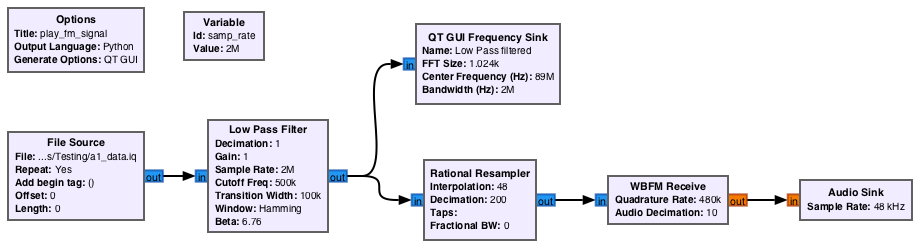
\includegraphics[width=0.8\textwidth]{Images/diagrams/play_fm_signal.png}
    \caption{Flow graph for playback of FM signals from recorded IQ files using GNU Radio}
    \label{fig:fm-demod}
\end{figure}
The additional benefit of this was to analyse file size (a possible indication of time-aligned and synchronised sampling) and if there were time-alignment issues. Albeit that this is very course as microseconds difference would not be viewable. 

\newpage


%---------------------------------
% Summary
%---------------------------------
\section{Summary}
This chapter thoroughly explored the design of both the hardware and software used in this \gls{rdf} project. First, an overview of the simulation was presented and aimed to prove the theoretical workings of the implemented project. Second, a high-level overview of the system, with appropriate block diagrams and reference material was provided. Connection diagrams and hardware diagrams are used to convey the workings of hardware components. Short snippets of code were provided for the Software section and used to demonstrate the functionality of the code. For the main workings of the code, and non-trivial calculations, longer algorithms are shown. 

% ----------------------------------------------------
\ifstandalone
\bibliography{Bibliography/References}
\printnoidxglossary[type=\acronymtype,nonumberlist]
\fi
\end{document}
% ----------------------------------------------------